\documentclass[../Main.tex]{subfiles}
% For a more professional table, add this to your main preamble: \usepackage{booktabs}

\begin{document}

\section*{Introduction}
\addcontentsline{toc}{section}{Introduction}

This chapter provides the institutional context for the research presented in this report. It begins by introducing Mohammed VI Polytechnic University (UM6P) as a leading African institution dedicated to applied research and innovation. Subsequently, it details the mission and structure of Ai movement, Morocco's International Center for Artificial Intelligence (AI), which is affiliated with UM6P. The center serves as the direct environment for this research internship, providing the necessary resources, expertise, and strategic direction. The following sections will detail the history, mission, and key initiatives of both institutions.

\section{Mohammed VI Polytechnic University}
Mohammed VI Polytechnic University (UM6P) is a non-profit private research university located in Benguerir, Morocco. With a strong focus on African development, the university prioritizes applied research and innovation to contribute to regional economic and human advancement. Officially inaugurated in 2017, UM6P has rapidly become a leading research institution, fostering interdisciplinary collaboration and facilitating strategic partnerships between Africa, Europe, and the rest of the world. As illustrated in Figure~\ref{fig:um6p_logo}, the university embodies Morocco's commitment to education and the knowledge economy.

\begin{figure}[H]
    \centering
    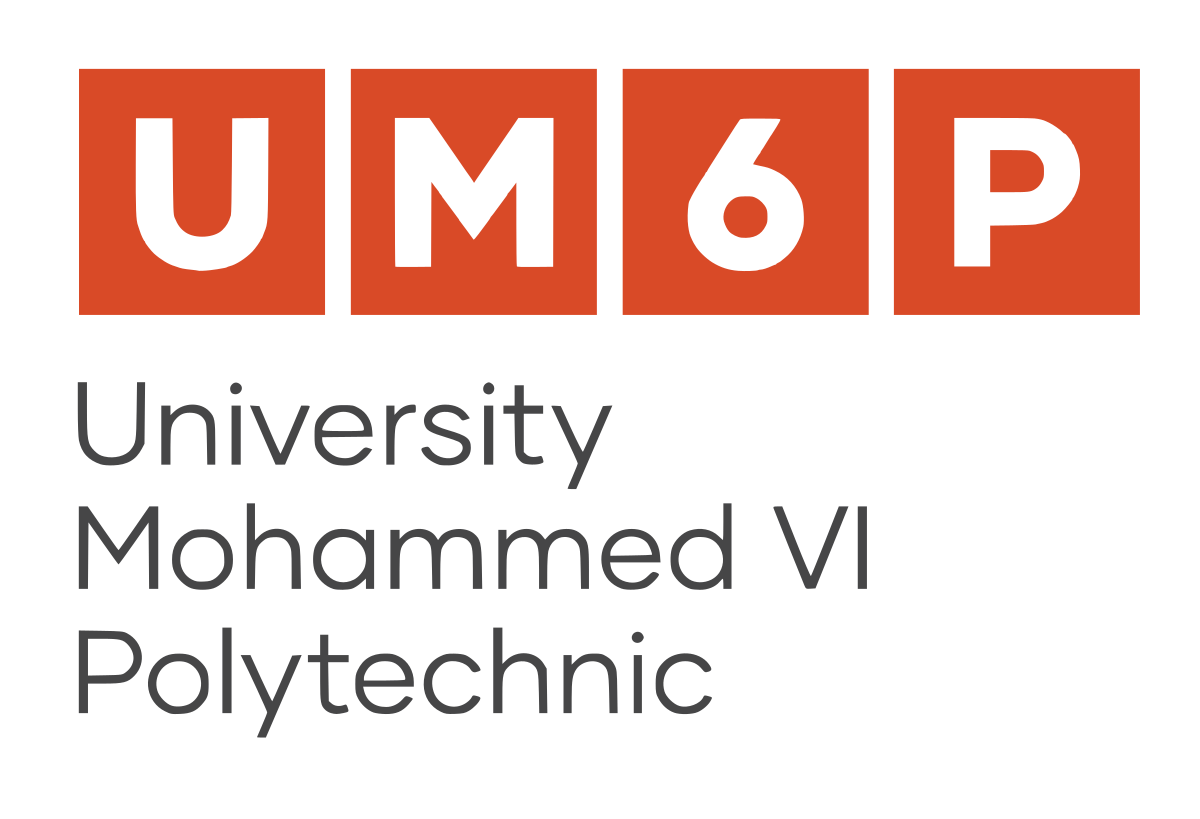
\includegraphics[width=0.3\textwidth]{img/logo/um6p.png}
    \caption{The official logo of Mohammed VI Polytechnic University.}
    \label{fig:um6p_logo}
\end{figure}

\textbf{History and Strategic Mission}
Established as part of the "Green City" urban development project, UM6P began operating in 2013. Its creation reflects a national vision to promote higher education and innovation as primary drivers of progress. The university is home to the most powerful supercomputer in Africa, the African Supercomputing Center, which provides a significant advantage for data-intensive research.

UM6P's mission is multifaceted, encompassing the development of competent leaders, the promotion of impactful research, and the cultivation of social responsibility and sustainable development. It hosts 5,684 students from over 20 nationalities and maintains numerous international partnerships with prestigious institutions such as the Massachusetts Institute of Technology, Columbia Business School, and HEC Paris. Its key faculties include the School of Agriculture, the Africa Business School, and the Institute of Science, Technology \& Innovation, among others.

\section{Ai movement: Morocco's International Center for Artificial Intelligence}
Affiliated with UM6P, Ai movement is Morocco’s International Center for Artificial Intelligence. It was established to be a continental leader in the field, dedicated to growing Moroccan and African talent, solving complex problems with innovative and ethical solutions, and building the next generation of leaders in artificial intelligence and data sciences.

\begin{figure}[H]
    \centering
    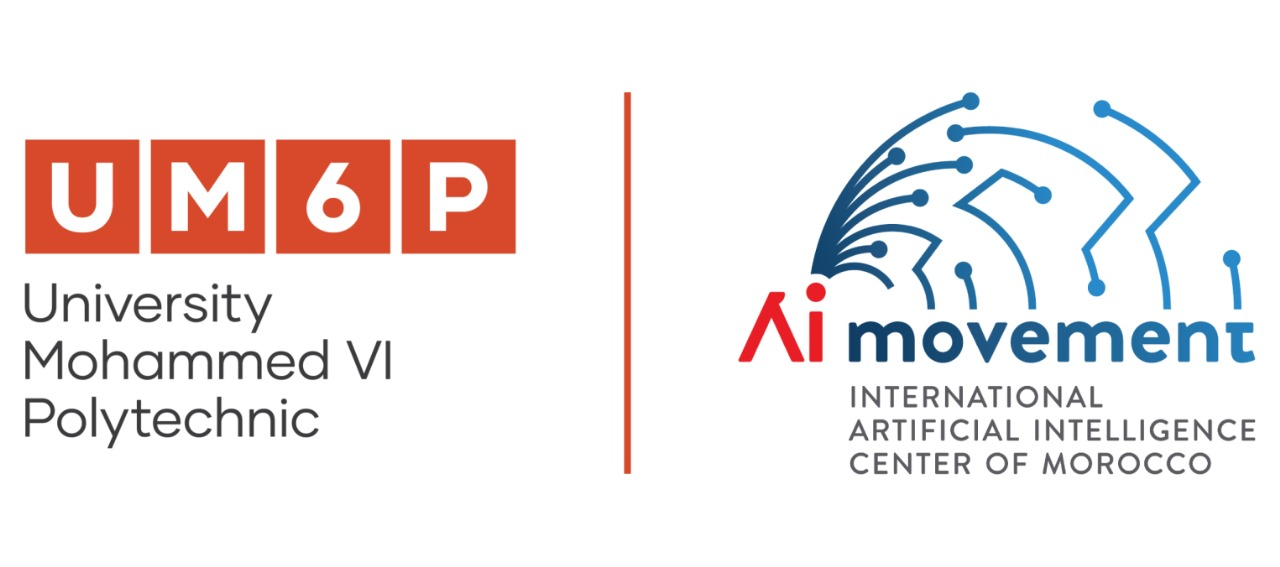
\includegraphics[width=0.65\textwidth]{img/logo/aim-um6p.jpeg}
    
\includegraphics[width=0.27\textwidth]{img/logo/unesco.jpeg}
    \caption{Logo Ai movement.}
\end{figure}


\subsection{Mission and Vision}
The center serves a dual role: it is both a coordinating platform for consolidating national AI-related initiatives and a proactive force for guiding the transformations associated with the field. Its mission is to deliver operational, resilient, and ethical solutions to pressing societal, environmental, and economic challenges. This vision is articulated by Pr. Amal El Fallah Seghrouchni, the Executive President of Ai movement:
\begin{quote}
    ”Within Mohammed VI Polytechnic University, we have created the Moroccan International Center of Artificial Intelligence called the Ai movement. In order to accompany the transformations induced by the advent of Artificial Intelligence and Data Sciences, to promote the emergence of a Moroccan and African know-how, and to meet the many challenges raised by AI... Our center promotes a hybrid and integrative approach to build deep AI and full stack of AI systems taking advantage of the complementarity of different AI paradigms.”
\end{quote}

The technical specifications of the center are summarized in Table~\ref{tab:aim_data}.

\begin{table}[H]
\centering
\caption{Technical data for the Ai movement center.}
\label{tab:aim_data}
\begin{tabular}{@{}ll@{}}
\toprule
\textbf{Attribute} & \textbf{Detail} \\ \midrule
\textbf{Center Name} & Ai movement \\
\textbf{Date of Establishment} & 11th November, 2022 \\
\textbf{Headquarters} & Rabat, Morocco \\
\textbf{Management} & Dr. Btissam El Khamlichi \\
\textbf{Products} & AI solutions, innovative software, and algorithms \\
& for data analysis and machine learning. \\ \bottomrule
\end{tabular}
\end{table}

\subsection{Key Partnerships and Recognition}
The strategic importance of Ai movement is underscored by its key partnerships and international recognition, as depicted in Figure~\ref{fig:aim_partners}. In a landmark decision, the United Nations Educational, Scientific and Cultural Organization (UNESCO) granted Ai movement Category II status, making it the first such center for artificial intelligence in Africa. This designation recognizes it as a regional hub of expertise that provides technical assistance and services to member states.

Furthermore, the center was founded in partnership with OCP Group (formerly Office Chérifien des Phosphates), Morocco's global leader in the phosphate and fertilizer industry. This partnership represents a significant investment in technology and energy transition, positioning the center at the forefront of applied AI research in strategic sectors.


\begin{figure}[H]
    \centering
    \begin{subfigure}[b]{0.7\textwidth}
        \centering
        % 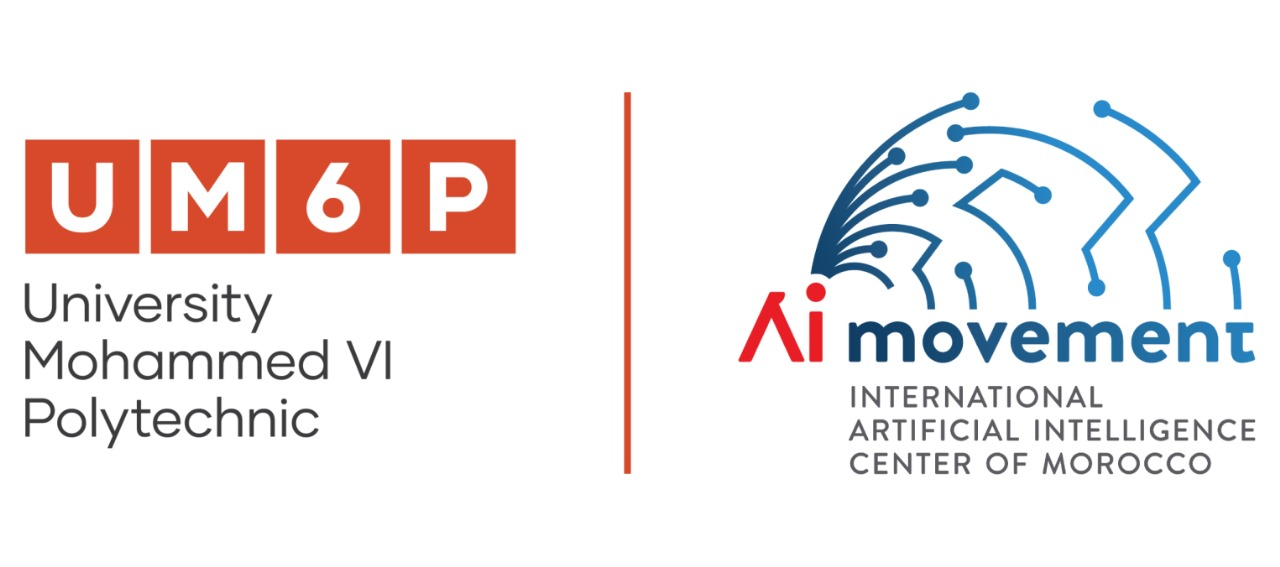
\includegraphics[width=\linewidth]{img/logo/aim-um6p.jpeg}
        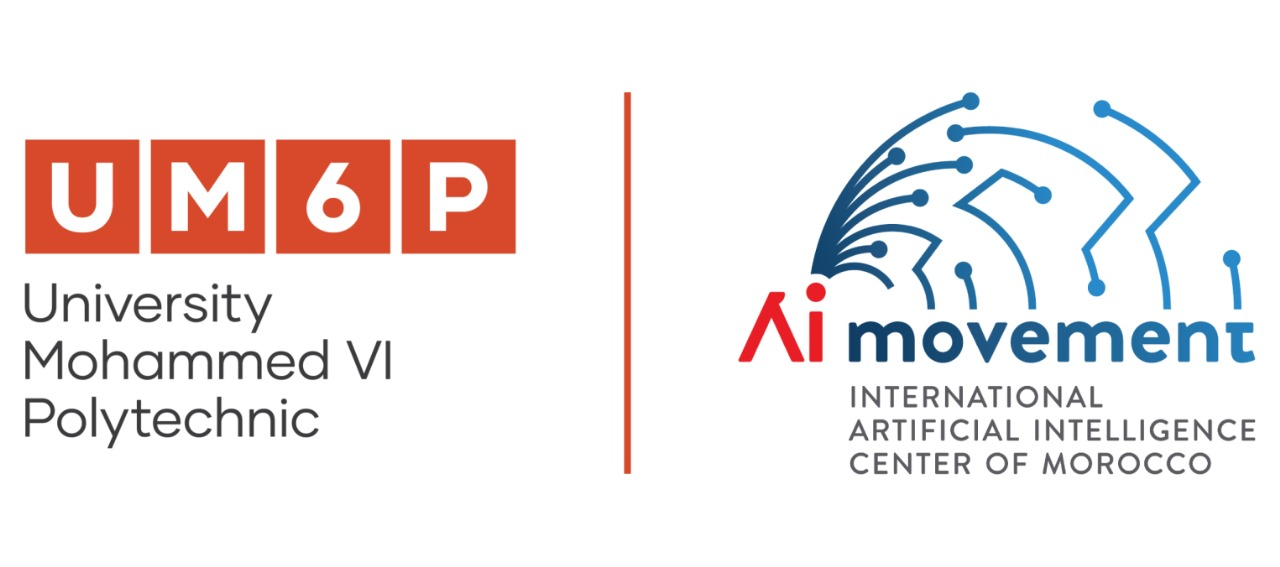
\includegraphics[width=0.65\textwidth]{img/logo/aim-um6p.jpeg}
        
\includegraphics[width=0.27\textwidth]{img/logo/unesco.jpeg}
        \caption{Ai movement center logo.}
    \end{subfigure}
    \begin{subfigure}[b]{0.25\textwidth}
        \centering
        
\includegraphics[width=0.5\linewidth]{img/logo/ocp.png}
        \caption{Key partners: UNESCO and OCP Group.}
    \end{subfigure}
    \caption{The Ai movement center and its key strategic partners.}
    \label{fig:aim_partners}
\end{figure}


\subsection{Core Pillars and Objectives}
The initiatives at Ai movement are structured around several core pillars, illustrated in Figure~\ref{fig:aim_pillars}. The program aims to prepare leaders to responsibly drive AI projects by covering key technologies, managerial tools, and business-oriented use cases. Key objectives include:
\begin{itemize}
    \item Understanding different AI techniques and their industry-specific applications.
    \item Exploring advanced machine learning architectures for computer vision, language processing, and robotics.
    \item Acquiring governance skills for trusted AI, including data management, regulation, and ethics.
    \item Developing an attractive ecosystem through international collaborations and local talent development.
\end{itemize}
One of UM6P’s prominent research laboratories contributing to this mission is MSDA, which stands for Modeling, Simulation, and Data Analysis. This lab specializes in the mathematical and analytical foundations that underpin many advanced AI systems.

\begin{figure}[H]
    \centering
    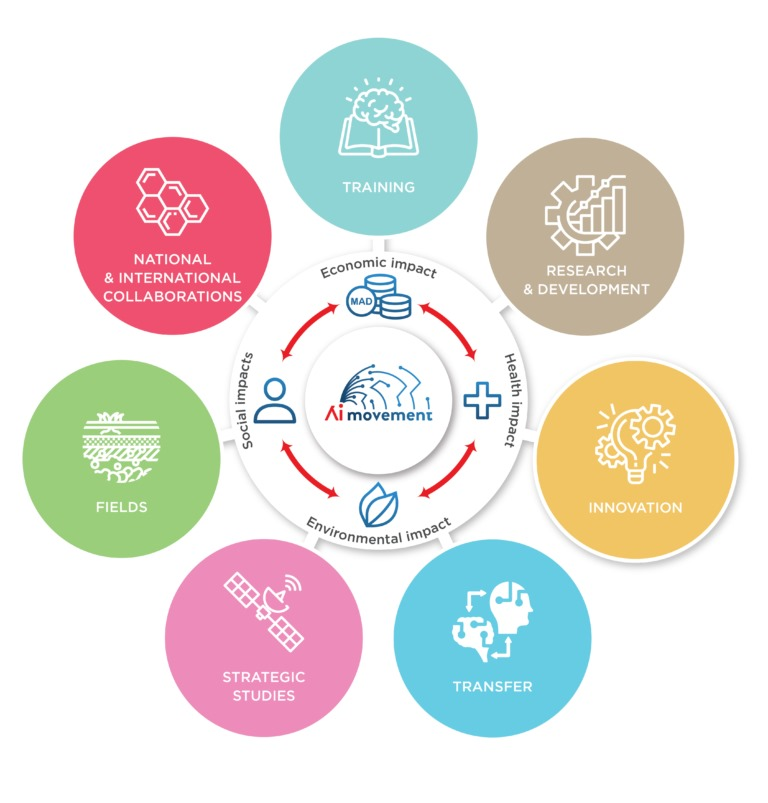
\includegraphics[width=0.6\textwidth]{img/aim-pillars.jpeg}
    \caption{The strategic pillars of the Ai movement center.}
    \label{fig:aim_pillars}
\end{figure}

\section*{Conclusion}
\addcontentsline{toc}{section}{Conclusion}

This chapter has detailed the institutional framework in which this research was conducted. Mohammed VI Polytechnic University provides a foundation of academic excellence and a commitment to innovation on the African continent. Within this dynamic environment, the Ai movement center offers a specialized, world-class hub for artificial intelligence research, talent development, and the creation of ethical, impactful solutions. This rich ecosystem of expertise and resources forms the ideal setting for the advanced deep reinforcement learning project detailed in the subsequent chapters of this report.

\end{document}
